\section{Prerequisites}

\begin{frame}{Analog In Memory Computing}
  \begin{itemize}
    \setlength{\itemsep}{6pt}
    \item Multiplication computation done via Ohm's Law:
          \begin{equation}
            I = \frac{V}{R}
          \end{equation}
    \item Voltage $V$, current $I$ and resistance $R$.
    \item Possible to rewrite resistance as conductance $G$:
          \begin{equation}
            I = G V \quad \text{with} \quad G = \frac{1}{R}
          \end{equation}
    \item Addition done via Kirchhoff's Law for any connected node in a circuit:
          \begin{equation}
            \sum_{n=0}^{N} I_n = 0 \;\rightarrow\; I_0 = - \sum_{n=1}^{N} I_n
          \end{equation}
    \item Currents can be trivially added by simply connecting electric lines.
  \end{itemize}
\end{frame}

\begin{frame}{The ``Memristor''}
  \begin{columns}[c]
    \begin{column}{0.52\textwidth}
      \textbf{Program weights by setting the resistance}:
      \begin{itemize}
        \setlength{\itemsep}{3pt}
        \item Apply $-V > -V_S \;\rightarrow$ set to low resistance
        \item Apply $\phantom{-}V > \phantom{-}V_R \;\rightarrow$ set to high resistance
        \item Intermediate states possible
        \item State is physically stored (non-volatile memory)
      \end{itemize}
      \vspace{0.4cm}
      \textbf{Problems}:
      \begin{itemize}
        \setlength{\itemsep}{3pt}
        \item Resulting resistance state varies with each programming cycle
        \item Non-linear relation of current and voltage
      \end{itemize}
    \end{column}

    \begin{column}{0.48\textwidth}
      \centering
      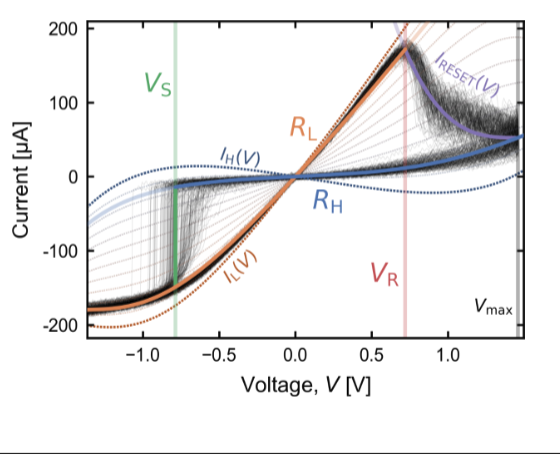
\includegraphics[width=\linewidth]{figures/memristor_iv_curve.png}
    \end{column}
  \end{columns}
\end{frame}

\begin{frame}{Memristor Array (1)}
  \begin{columns}[c]
    \begin{column}{0.54\textwidth}
      \begin{itemize}
        \setlength{\itemsep}{4pt}
        \item Memristors as connecting element between vertical and horizontal circuit lines
        \item Each memristor is a weight of a matrix
        \item Column sum via simple line connection
        \item Weight matrices are typically fixed during application
      \end{itemize}
      \vspace{0.3cm}
      \textbf{Problems}:
      \begin{itemize}
        \setlength{\itemsep}{3pt}
        \item Only positive, non-zero weights possible
        \item Current leakage prohibits a true zero
      \end{itemize}
    \end{column}

    \begin{column}{0.46\textwidth}
      \centering
      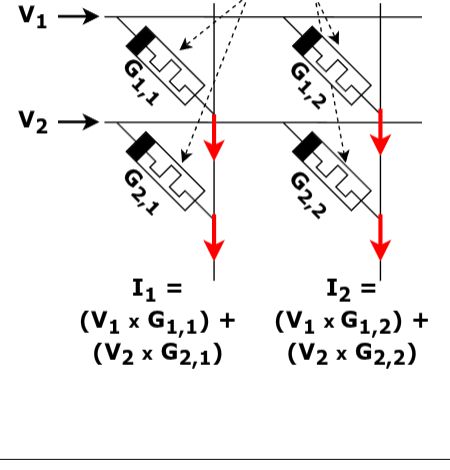
\includegraphics[width=\linewidth]{figures/memristor_array_1.png}
    \end{column}
  \end{columns}
\end{frame}

\begin{frame}{Memristor Array (2)}
  \begin{columns}[c]
    \begin{column}{0.50\textwidth}
      \begin{itemize}
        \setlength{\itemsep}{3pt}
        \item Use positive and negative bitlines to create memristor pairs
        \item Each row-wise pair of memristors represents a weight
        \item[$\rightarrow$] Differential pair allows for negative and zero weight values:
              \begin{equation*}
                I_j = \sum_{i=1}^{N} V_i G_{i,j}^{+} - \sum_{i=1}^{N} V_i G_{i,j}^{-}
              \end{equation*}
      \end{itemize}
      \vspace{0.2cm}
      \textbf{Problems}:
      \begin{itemize}
        \setlength{\itemsep}{3pt}
        \item Cannot set paired memristors to identical conductances
        \item[$\rightarrow$] Results close to zero, but not guaranteed
      \end{itemize}
    \end{column}

    \begin{column}{0.50\textwidth}
      \centering
      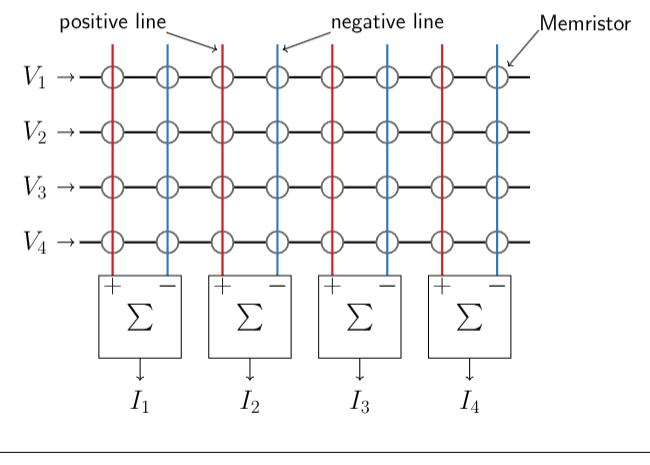
\includegraphics[width=\linewidth]{figures/memristor_array_2.png}
    \end{column}
  \end{columns}
\end{frame}

\begin{frame}{Non-Idealities and Synaptogen}
  \begin{itemize}
    \setlength{\itemsep}{5pt}
    \item Ideal crossbars are assumed by many simulators; real devices exhibit:
          \begin{itemize}
            \item Device-to-device and cycle-to-cycle programming variability
            \item Thermal (Johnson--Nyquist) noise
            \item Finite DAC/ADC resolution
            \item Imprecise intermediate (non-binary) conductance levels
          \end{itemize}
    \item Synaptogen \cite{hennen2024synaptogen}: generative device model based on a
          vector autoregression, fitted to 3M+ measured programming cycles of
          130\,nm memristors (STMicroelectronics).
    \item In our experiments (PyTorch, SynaptogenML): linear layers are replaced by
          crossbar simulation, the rest of the network stays conventional.
  \end{itemize}
\end{frame}

\begin{frame}{Quantization-Aware Training}
  \begin{itemize}
    \setlength{\itemsep}{6pt}
    \item Memristor execution effectively means: low-precision (stacked binary) weights
          + 8-bit DAC/ADC on activations.
    \item Post-training quantization (PTQ) collapses at low precision;
          quantization-aware training (QAT) \cite{gholami2021survey} inserts
          fake quantization into the training from epoch 1.
          \begin{itemize}
            \item Symmetric per-tensor quantization, zero-point fixed to 0
                  (required by the pairwise encoding).
          \end{itemize}
  \end{itemize}
  \vfill
  \begin{table}[h]
    \centering
    \caption{WER (\%) on TED-LIUMv2 dev, Conformer CTC, 4-gram LM
      \cite{rossenbach2025memristor}. Memristor: mean $\pm$ std over 10
      differently programmed devices.}
    \label{tab:anchor-results}
    \small
    \begin{tabular}{l c c c c c c c}
      \toprule
      Weight bits           & FP32 & 8   & 6   & 5   & 4    & 3    & 2    \\
      \midrule
      PTQ                   & 7.2  & 7.2 & 7.9 & 8.9 & 11.4 & 30.7 & --   \\
      QAT                   &      & 7.3 & 7.7 & 7.4 & 7.8  & 8.3  & 22.1 \\
      Memristor (simulated) &      & 8.3 & 8.3 & 8.3 & 8.9  & 9.2  & --   \\
      \bottomrule
    \end{tabular}
  \end{table}
  \vfill
  \begin{itemize}
    \item Up to 3-bit weights: $\leq 25\%$ relative WER degradation on device
          ($9.2$ vs.\ $7.2$).
  \end{itemize}
\end{frame}
